\section{Padrões de Feedback}

\begin{frame}{Padrões de Feedback}
\begin{block}{Mensagens de Erros}
  \begin{itemize}
    \item<1-> As mensagens de erros devem ser expressas em linguagem simples, para indicar precisamente o problema e sugerir construtivamente uma solução. 
  \end{itemize}
\end{block}
\end{frame}
%%%%%%%%%%%%%%%%

\begin{frame}{Padrões de Feedback}
\begin{block}{Mensagens de Erros}
  \begin{itemize}
    \item<1-> \begin{figure}[\center]
    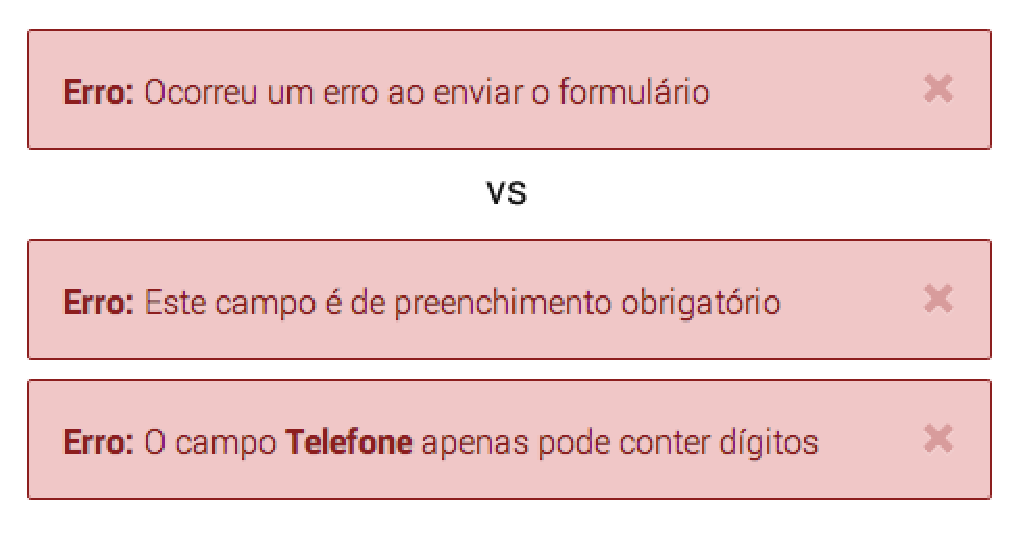
\includegraphics[width=5cm]{figuras/error/msg_error}
    \end{figure}
  \end{itemize}
\end{block}
\end{frame}
%%%%%%%%%%%%%%%%

\begin{frame}{Padrões de Feedback}
\begin{block}{Mensagens de Erros}
  \begin{itemize}
    \item<1-> \begin{figure}
    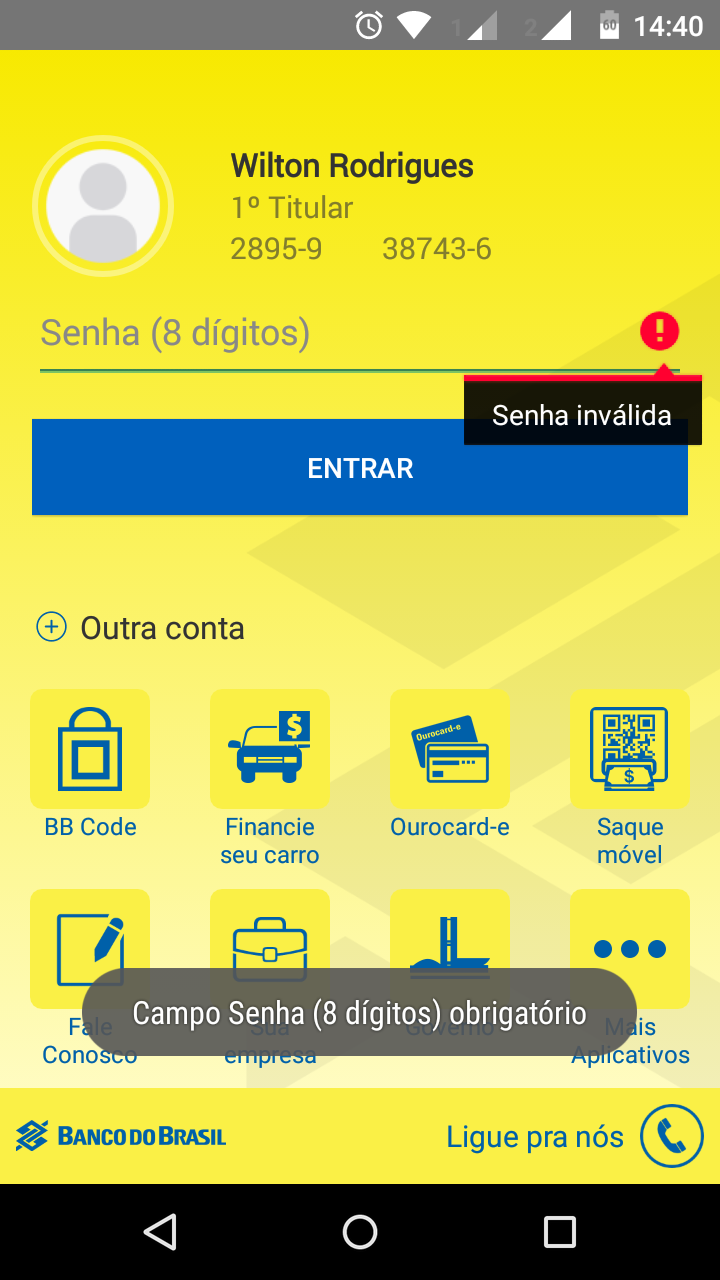
\includegraphics[width=3cm]{figuras/error/error2}
    \end{figure}
  \end{itemize}
\end{block}
\end{frame}
%%%%%%%%%%%%%%%%

\begin{frame}{Padrões de Feedback}
\begin{block}{Mensagens de Erros}
  \begin{itemize}
    \item<1-> \begin{figure}
    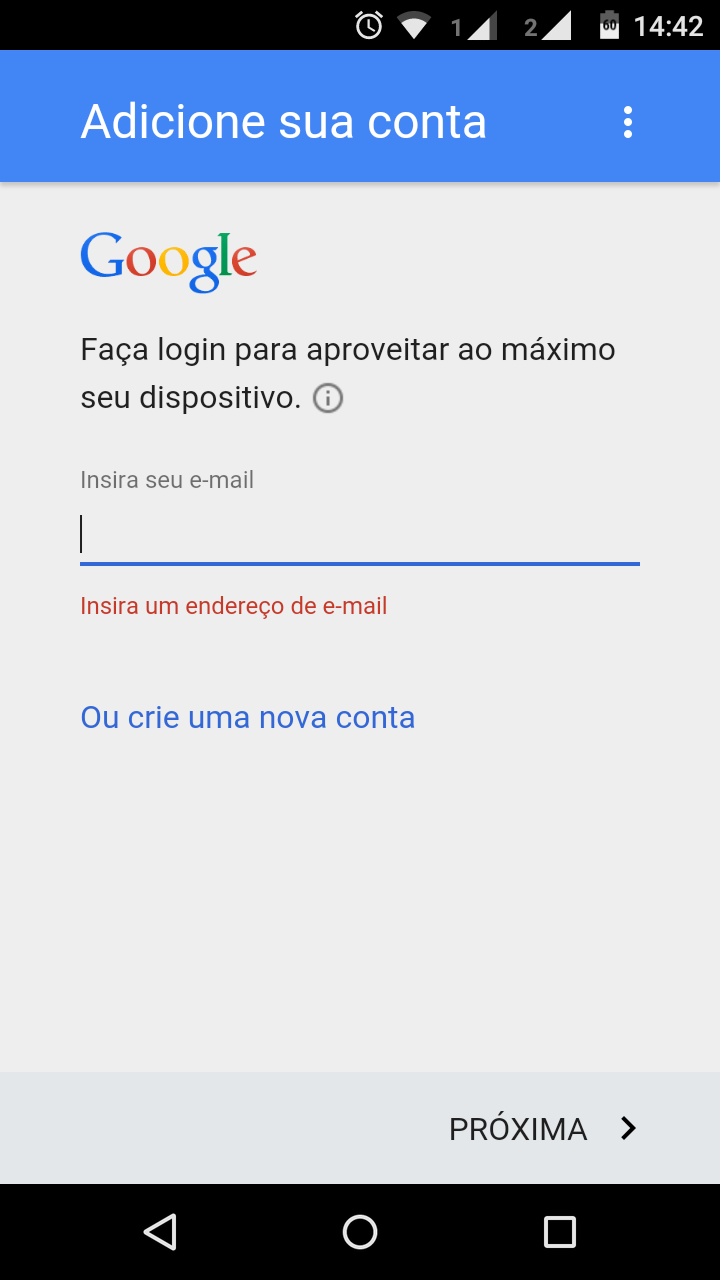
\includegraphics[width=3cm]{figuras/error/error3}
    \end{figure}
  \end{itemize}
\end{block}
\end{frame}
%%%%%%%%%%%%%%%%

\begin{frame}{Padrões de Feedback}
\begin{block}{Mensagens de Erros}
  \begin{itemize}
    \item<1-> \begin{figure}
    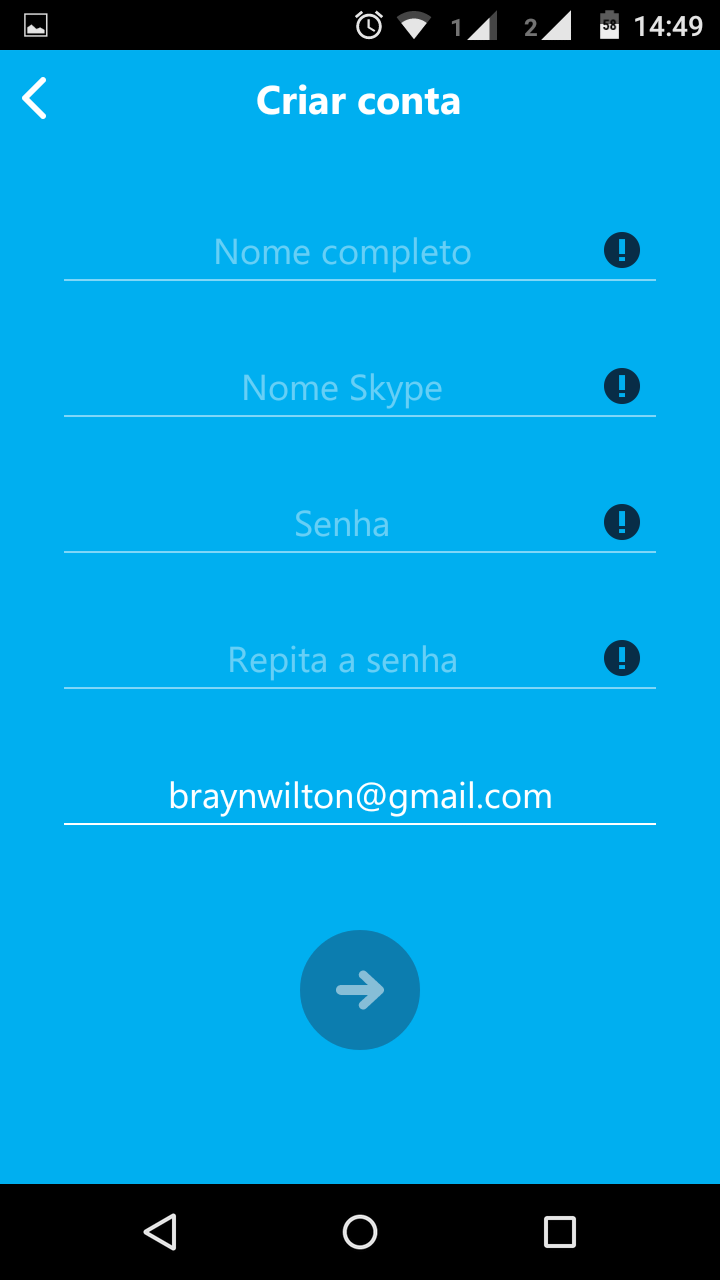
\includegraphics[width=3cm]{figuras/error/error4}
    \end{figure}
  \end{itemize}
\end{block}
\end{frame}
%%%%%%%%%%%%%%%%

\begin{frame}{Padrões de Feedback}
\begin{block}{Mensagens de Erros}
  \begin{itemize}
    \item<1-> \begin{figure}
    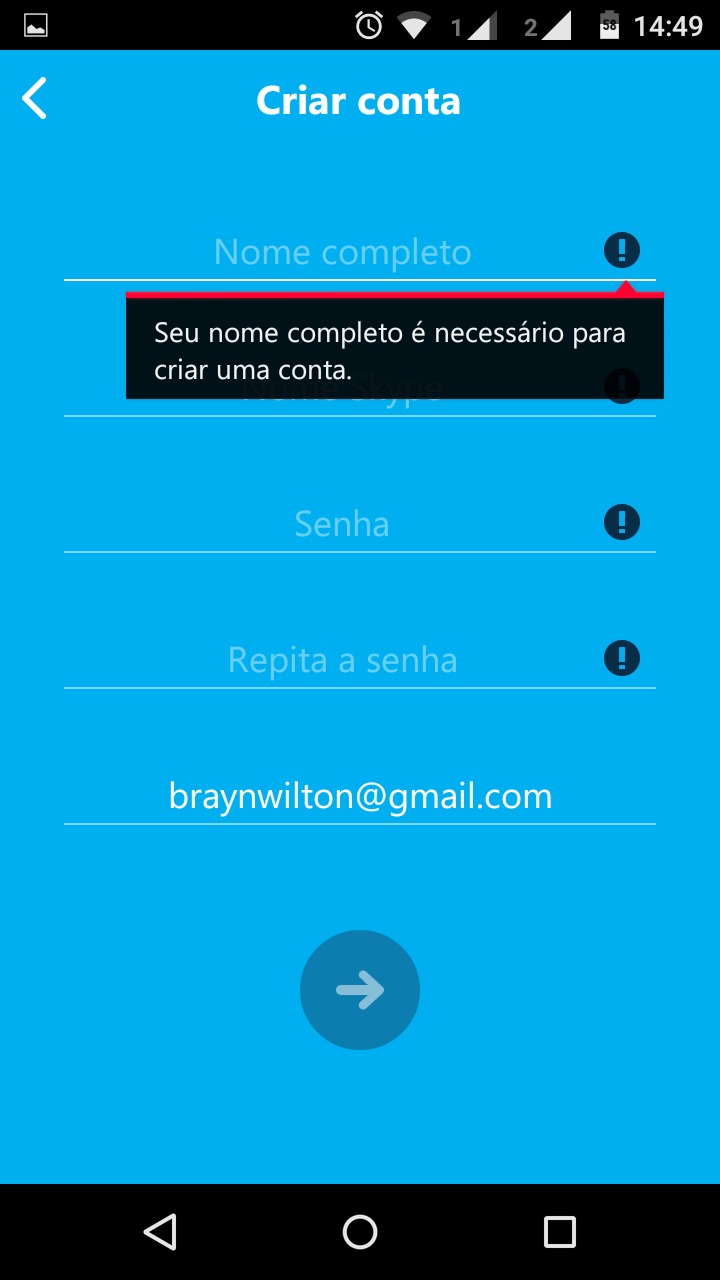
\includegraphics[width=3cm]{figuras/error/error5}
    \end{figure}
  \end{itemize}
\end{block}
\end{frame}
%%%%%%%%%%%%%%%%

\begin{frame}{Padrões de Feedback}
\begin{block}{Mensagens de Confirmação}
  \begin{itemize}
    \item<1-> As mensagens de confirmação devem ser exibidas sempre que uma ação é realizada. Mas de forma que as mensagens não interrompam o fluxo do usuário.
  \end{itemize}
\end{block}
\end{frame}
%%%%%%%%%%%%%%%%

\begin{frame}{Padrões de Feedback}
\begin{block}{Status do Sistema}
  \begin{itemize}
    \item<1-> As mensagens de status do sistema aumentar a confiança dos usuários na aplicação. Pois elas informam qual o estado da aplicação impedindo que o usuário fique imaginando se a aplicação travou.
  \end{itemize}
\end{block}
\end{frame}
%%%%%%%%%%%%%%%%

\begin{frame}{Padrões de Feedback}
\begin{block}{Status do Sistema}
  \begin{itemize}
    \item<1-> \begin{figure}
    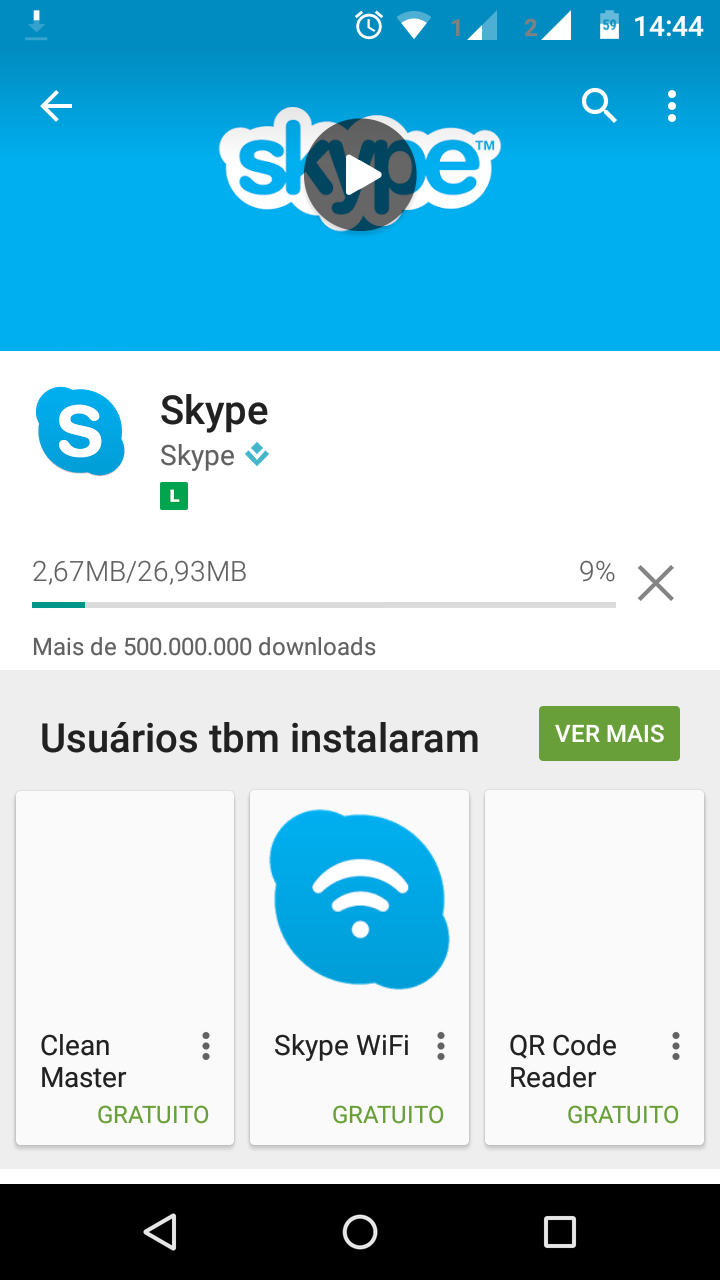
\includegraphics[width=3cm]{figuras/status/status}
    \end{figure}
  \end{itemize}
\end{block}
\end{frame}
%%%%%%%%%%%%%%%%

\begin{frame}{Padrões de Feedback}
\begin{block}{Status do Sistema}
  \begin{itemize}
    \item<1-> \begin{figure}
    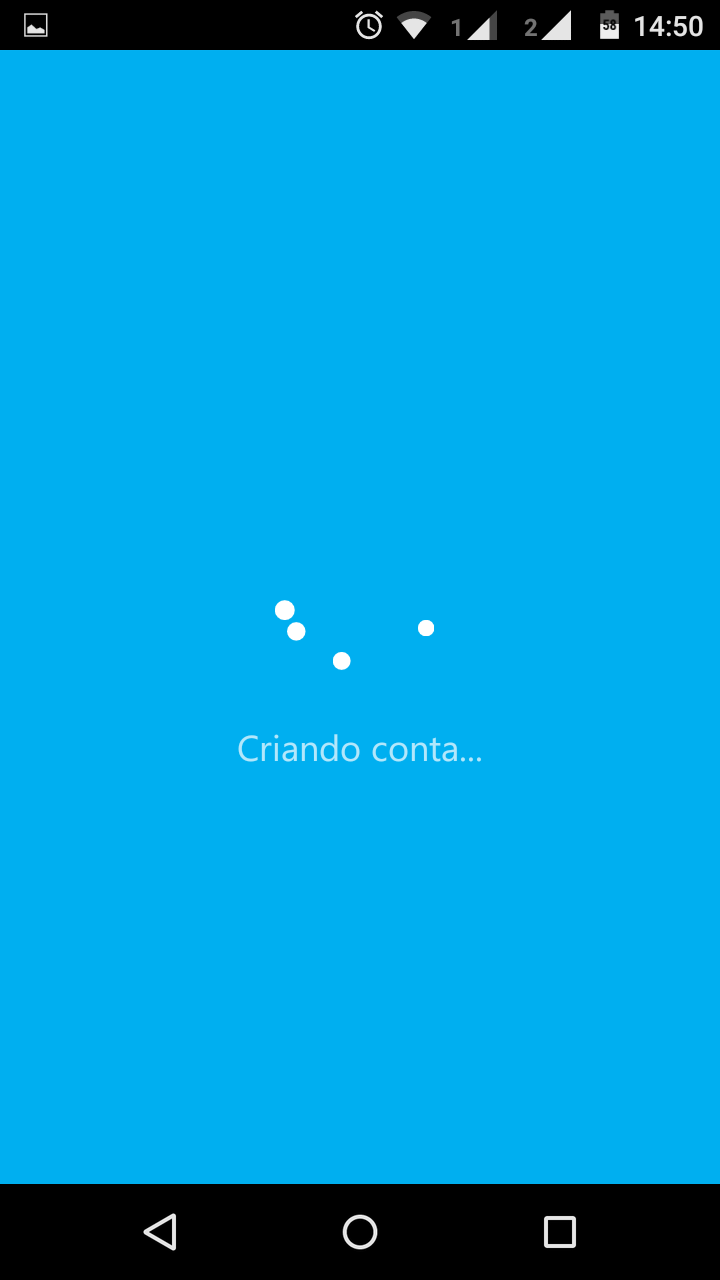
\includegraphics[width=3cm]{figuras/status/status1}
    \end{figure}
  \end{itemize}
\end{block}
\end{frame}
%%%%%%%%%%%%%%%%

\begin{frame}{Padrões de Feedback}
\begin{block}{Status do Sistema}
  \begin{itemize}
    \item<1-> \begin{figure}
    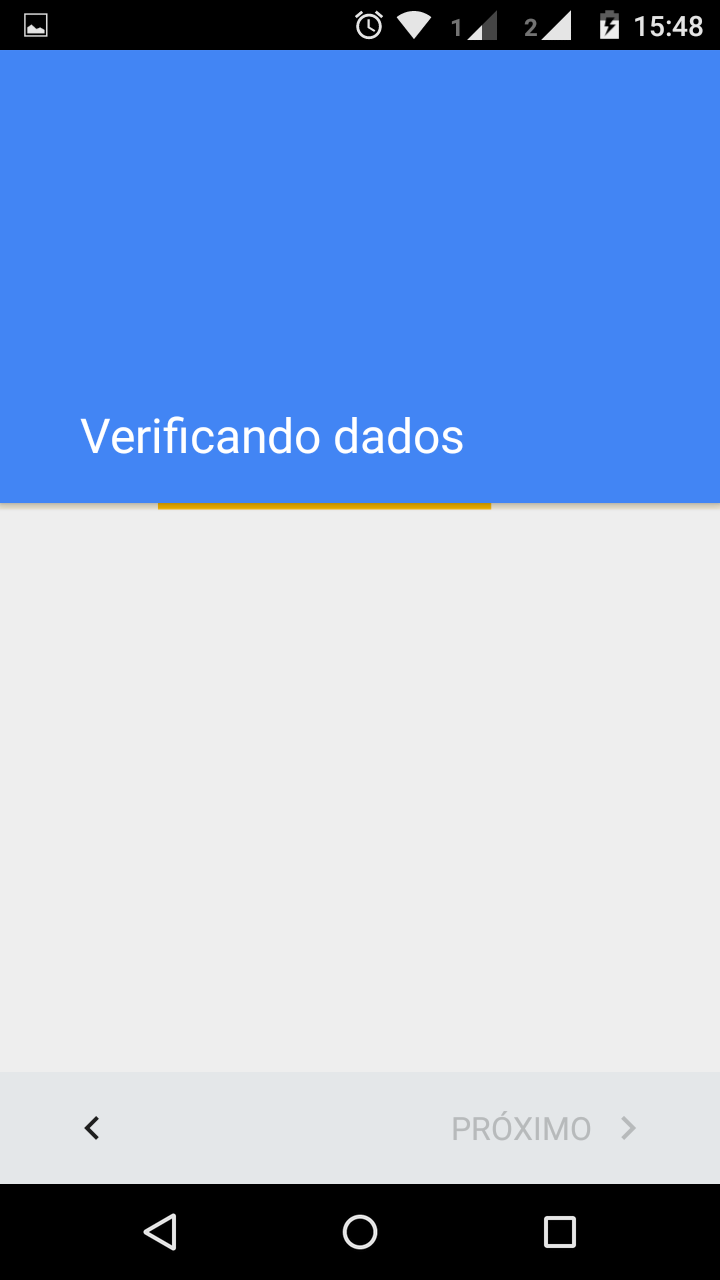
\includegraphics[width=3cm]{figuras/status/status2}
    \end{figure}
  \end{itemize}
\end{block}
\end{frame}
%%%%%%%%%%%%%%%%